\section{Communicating with the satellite}

\begin{figure}
  \begin{center}
    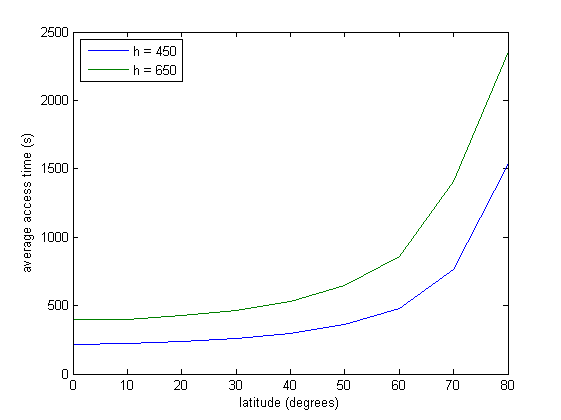
\includegraphics[width=1.0\textwidth]{Figures/accesstid450og650}
  \end{center}
  \caption[Accesstid for 450 og 650]{Access times for $h=450km$ and $h=650km$ as a function of ground station latitude}
  \label{fig:acctid}
\end{figure}

Since we don't know when the satellite will be launched we don't know the exact orbit. The project manager, Roger Birkeland, told us that we can assume the orbit will  have a height above the Earth somewhere between 450km and 650km and inclination of 98 degrees. The uncertainty in $h$ is critical, because the height above the earth dramatically changes the access time of a ground station, see Fig. \ref{fig:acctid}. 

\begin{figure}
  \begin{center}
    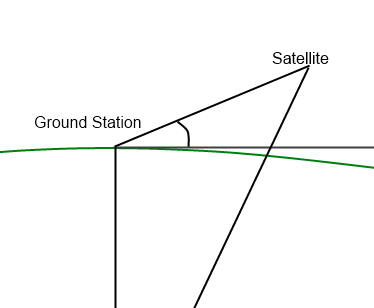
\includegraphics[width=0.7\textwidth]{Figures/groundstation_satelitte_geometry}
  \end{center}
  \caption[Ground station satellite geometry]{Illustration of geometry between a ground station and a satellite}
  \label{fig:gs_s_geom}
\end{figure}

The ground station can only communicate with a satelitte when it has a certain elevation. Which may depend on topology, atmosphere, antenna ...
In the following we assume that the minimum elevation is 25 degrees, maximum elevation is 90 degrees and no constraints on the azimuth angle.  For a illustration see Fig. \ref{fig:gs_s_geom}.

\begin{figure}
  \begin{center}
    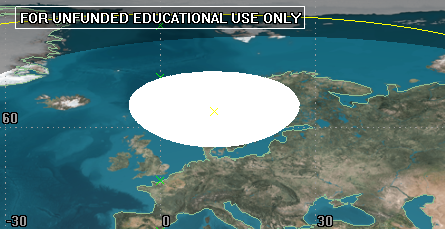
\includegraphics[width=0.8\textwidth]{Figures/ntnu_footprint}
  \end{center}
  \caption[ntnu footprint]{NTNU ground station range}
  \label{fig:ntnu_range}
\end{figure}

The result of this is that the ground station can communicate with the satelitte whenever the ground track is inside a rough circle centered on the ground station, see Fig. \ref{fig:ntnu_range} for the estimated "range" of the ground station at Gløshaugen operating with these constraints.

The Gløshaugen ground station will on average be able to communicate with the satellite 540 seconds per day if $h=450$ and 980 seconds per day if $h=650$. We don't know exactly how much data we need to download, but according to \cite{eks-kom} we'll need roughly 12 minutes (720 seconds) to download a single image. 

\subsection{Other ground stations}
Fig. \ref{fig:acctid} shows that the access time for a (near) polar satellite is nearly constant for ground stations at latitudes below 45 degrees. The access times of a ground station those low latitudes is in the 300 to 500 second range, i.e. about half a image, so we'll need about 2 ground stations at lower latitudes to download a single image. We may compare this to a single ground station located in Longyearbyen (78' N) which has a access time in the 1400 to 2300 second range, i.e. 2-3 images per day. 
